\chapter{Implementation and testing}

\section{Connecting to a MySQL server and executing queries} \label{ch:impllib:sec:connecting}
To connect to a MySQL server, the application uses the Ruby library mysql2. The library, or gem as it's called in Ruby, provides the implementation for connecting, querying and retrieving results from a MySQL server. mysql2 is a binding to MySQL's C library libmysql. mysql2 is the more modern and lean version of the mysql version. Compared to mysql gem, mysql2 gem can be 2 times faster and is built with Ruby in mind. Furthermore, mysql2 is also much more popular with over 42 million downloads on RubyGems, compared to mysql's 8 million downloads.

To connect to a MySQL server, the library requires the address and port of the server, and an account and password. The account must be the root user or at least one that has the permission to create and drop databases, to create and drop users, and to grant permissions to an user.

\subsection{Handling concurrent submissions}

As the library will be used in a web application, concurrency is inevitable. Users can submit solutions at any time and it is possible that two users submit solutions at the same time. Obviously, concurrency can be ignored by limiting the execution of only one compile or assessment at a time. However, this solution can lead to frustrating waiting times and requires the implementation of background workers to compile the work. Therefore, the tool opted to implement a solution that allows concurrent executions.

To allow concurrency, each submission or compilation is performed using different connections to different databases (a MySQL server can have multiple databases).  Every compilation or submission begins by creating a new and unique database based on the current time. The database name will follow the format \texttt{HOURMINUTESECOND}. While this should cover most cases, due to the concurrent nature of the application, it might be the case that two connections try to create a database with the same name. However, MySQL statements are atomic. That means that two statements can not both change the schema of the MySQL server. Therefore, it is guaranteed that at least one create will fail. In this case, we repeat all failed creations (by using the new time) until they succeed. On second and further attempts, we also add a \mintinline{ruby}{_attempt} at the end of the database name to reduce the chance of another conflict. At the end of the compilation, the newly created database will be dropped and all data associated discarded.

%TC:ignore
\begin{listing}
    \centering
    \begin{minted}{ruby}
success = false
attempt = 0
while !success do
  time = DateTime.now

  if attempt > 0
    @database = "#{Time.now.strftime("%H%M%S")}_#{attempt}"
  else
    @database = "#{Time.now.strftime("%H%M%S")}"
  end

  begin
    @client.query("CREATE DATABASE `#{@database}`")
    success = true
  rescue Mysql2::Error => exception
    raise exception unless exception.message.include?("database exists")
    success = false
    attempt += 1
  end
end
\end{minted}
    \caption{Creating a new database for each run}
    \label{fig:creating_new_database}
\end{listing}
%TC:endignore

\subsection{Preventing malicious actions from input SQL queries}

Considering the fact that the library executes arbitrary queries, the risks associated with malicious SQL are significant. The application never returns back the query results which means that the potential for data leaking through this does not exist. However, an arbitrary query can destroy or modify other databases on the MySQL server. Therefore, the library must take extra precautions as it deals with unchecked user code. To prevent malicious actions, we create a new MySQL user that only has permission for the newly created database.
%TC:ignore
\begin{listing}
\begin{minted}{ruby}
@client.query("CREATE USER IF NOT EXISTS `#{@database}`;")
@client.query("GRANT ALL PRIVILEGES ON `#{@database}`.* TO `#{@database}` WITH GRANT OPTION;")
\end{minted}
\caption{Creating a new user with permissions for the new database}
\label{fig:creating_new_user}
\end{listing}
%TC:endignore
All used queries are performed using this user, instead of using the root one. The temporary user is also deleted at the end of the compile/ assessment execution. This way, the user input can only damage the created database for his assessment. However, this is not an issue considering these are short-lived databases which are destroyed at the end of the assessment.

The only way to get around the limitation of the restricted user would be to use a different user. Changing the user in MySQL is not possible through a MySQL command. The only possible way would be to use the \texttt{system} command which executes bash code in combination with the \texttt{mysql -uroot --password} bash command if they knew the root password, but not the url of the database. However, the \texttt{system} command is only available on connections opened with the \texttt{mysql} bash command, which is not the case for \texttt{mysql2} - so users can not exploit this method. Furthermore, the user has limited permissions so he can not run commands such as \mintinline{mysql}{SET PASSWORD} to change existing users.



\section{Parsing and transforming queries}

Part of the canonicalization and grading process, SQL queries will go through multiple transformations after being parsed and separated in independent components. MySQL does not provide an official parser for any programming language, so the library had to use a 3rd party tool.

The library initially used the Ruby gem sql-parser. Throughout the development process, there have been multiple problems associated with this tool. Most importantly, the library did not have support for multiple SQL statements that we required. Unfortunately, many issues with sql-parser were discovered only late in the project.

An alternative was represented by pg\_query Ruby gem. Internally it uses PostgreSQL's parsing library libpg\_query built in C++. pg\_query provides much better code and stability, due to its nature of being part of a production database system, compared to sql-parser which was only used for parsing. PostgreSQL, like MySQL, is a database system that is widely used, being the 4th most used database engine according to \cite{db_engine:statistics}. Although both PostgreSQL and MySQL have SQL at their core, each one implements their own version of SQL. Therefore, a query might work in MySQL, but not work in PostgreSQL, or return different results. For instance, in MySQL string comparison is case insensitive, while PostgreSQL is not. In addition, each SQL version adds their own functions that diverge from Standard SQL. Therefore, implementing pg\_query turned out to be impossible due to the many differences in syntax between them. In addition, time constraints made it unjustifiable to spend time on re-implementing all transformers already built.

\subsection{Extending sql-parser}

In the end, due to the issues described previously, a decision was made to continue using sql-parser. Fortunately, sql-parser uses a MIT license which allowed us to fork the library and implement the fixes in the fork. The parser was implemented using Racc's grammar files. According to the GitHub page of the tool, Racc is a \textit{LALR(1) parser generator} that generates Ruby code. LALR parsers are also known as "Look Ahead Left to Right" parsers. The fork created implemented the following functionality:
\begin{itemize}
    \item Support for \mintinline{mysql}{DISTINCT}, \mintinline{mysql}{DISTINCTROW}, \mintinline{mysql}{ALL} in \mintinline{mysql}{SELECT} statements
    \item Support for \mintinline{mysql}{LIMIT} and \mintinline{mysql}{OFFSET}
    \item Support for using a qualified column in \mintinline{mysql}{ORDER BY} clause
    \item Support for using the columns number in \mintinline{mysql}{GROUP} clause
\end{itemize}

The process of adding a new feature was formed of multiple parts:
\begin{enumerate}
    \item Create a \mintinline{ruby}{Node} class representing the new clause, if a new clause was implemented. A \mintinline{ruby}{Node} represents an element of a query: a number, a word, a condition, etc. For instance, the newly created \texttt{LIMIT} node has the following structure:
    \begin{listing}[H]\centering
\begin{minted}{ruby}
class LimitClause < Node
    def initialize(limit, offset)
        @limit = limit
        @offset = offset
    end

    attr_reader :limit, :offset
end
\end{minted}
\caption{Limit clause \mintinline{ruby}{Node}}
\label{fig:limit_clause}
\end{listing}
    \item Update existing \mintinline{ruby}{Node} to link to the newly created node. For instance, the \mintinline{ruby}{LimitClause} node had to be linked to the \mintinline{ruby}{TableExpression} node.
    \item Add the new parsing rules to Racc grammar file. For instance, when adding the LIMIT clause there are three options: there is only a limit number, there are two numbers for limit and offset separated by the word \texttt{OFFSET}, or the two numbers are separated by a comma:
\begin{listing}[H]
    \centering
    \begin{minted}{ruby}
  limit_clause
: # no action
| LIMIT unsigned_integer { result = SQLParser::Statement::LimitClause.new(val[1], nil) }
| LIMIT unsigned_integer OFFSET unsigned_integer { result = SQLParser::Statement::LimitClause.new(val[1], val[3]) }
| LIMIT unsigned_integer comma unsigned_integer { result = SQLParser::Statement::LimitClause.new(val[3], val[1]) }
    \end{minted}
    \caption{Limit clause \texttt{Racc}}
    \label{fig:limit_clause_racc}
\end{listing}
\end{enumerate}

\subsection{Using sql-parser to parse queries}

\subsection{Using sql-parser to change queries}
sql-parser also provides a way to change a parsed query (which is now a combination of multiple Nodes) back to a SQL query. Unfortunately, the process of internally modifying the structure of a query is not well-defined and there is no public interface exposed. Each node has one or more private instance variable that represent the values of the Node. For instance, the limit node shown in listing \ref{fig:limit_clause}, has two such variables: limit and offset. sql-parser does not provide a way to change these properties as all Nodes just expose a reader method (set using \mintinline{ruby}{attr_reader}). Fortunately, ruby provides a \mintinline{ruby}{instance_variable_set} method while allows anyone with a reference to an object to change that object's internal variables even if they are private and no setter is exposed. It is worth mentioning that while this approach might work, the use of this method \mintinline{ruby}{instance_variable_set} goes against the principle of encapsulation, and might mean that a future update to the library can lead to errors, if the internal structure of Nodes is modified.

\begin{listing}
\begin{minted}{ruby}
@parsed_query.query_expression.list.instance_variable_set(
  "@columns",
  new_columns
)
\end{minted}
\caption{Example of updating the column list for a parsed query}
\end{listing}

After a query is modified, sql-parser exposes a \mintinline{ruby}{.to_sql} method on each Node that can be used to transform a Node to a SQL statement.

\section{Canonicalizing queries}

As previously mentioned in section \ref{ch:lit:sec:improved_canon}, the library will implement a canonicalization step. The library implements all canonicalizations done by XData and described in section \ref{ch:lit:sec:canonicalization}, and the additional ones presented in section \ref{ch:lit:sec:improved_canon}. All transformations will use sql-parser's transformations ability combined with the ability to make queries on the database.

\subsection{Transforming \mintinline{mysql}{*} to all columns}
To transform \mintinline{mysql}{*} to MySQL, the library uses the fact that it doesn't need to support sub-queries. That means that it can simply look at what tables are selected and then perform \mintinline{mysql}{SHOW COLUMNS FROM table_name} on each table to get the full list of columns for each table. The library will then simply update the list of columns (initially represented by a \mintinline{mysql}{*}) to the new list of columns which contain the full list of \texttt{table\_name.column} for each selected table.

\begin{listing}
\begin{minted}{ruby}
new_columns = table_list.map do |table|
  columns_query = "SHOW COLUMNS from #{table}"
  columns = @connection.query(columns_query).map { |k| k["Field"] }

  columns.map do |column_name|
    SQLParser::Statement::QualifiedColumn.new(
      SQLParser::Statement::Table.new(table),
      SQLParser::Statement::Column.new(column_name)
    )
  end
end.flatten
\end{minted}
\caption{Getting the full list of columns for a query}
\end{listing}

\subsection{Transforming ambigous columns to unambigous columns}
Transforming ambiguous columns to unambiguous columns is done in a similar way as the previous transformations. The transformation makes use of two important aspects:
\begin{enumerate}
    \item One can determine the full list of columns for each table expression component, by running \mintinline{mysql}{SHOW COLUMNS FROM table_name}.
    \item An ambiguous column can belong to a single table from a query. If a column cannot be made qualified, then MySQL will automatically return the \textit{column xx in field list is ambiguous''} error.
\end{enumerate}

Therefore to transform an ambiguous column we must go through the full list of columns of each table until we find a match. We then transform the ambiguous column to a qualified column. This process can be seen in listing \ref{fig:find_table}.

An additional type of ambiguous column type is the position reference one which is found in the GROUP and ORDER clauses. In these two clauses, one can write \mintinline{mysql}{ORDER BY 2} where 2 references the second column from the select list. To find the qualified column that the position column references we need to look at the select list (after it was transformed to qualified columns) and select the right position: \mintinline{ruby}{@parsed_query.query_expression.list.columns[column.value - 1]} (position columns start at index 1, while arrays start at 0 in ruby)

Finally, the library also considers the aggregate column types which inside might contain a ambiguous column as well. Aggregate columns are of type \mintinline{ruby}{SQLParser::Statement::Aggregate} which has an attribute of type column. Therefore, we need to apply the same transformation to the inner column attribute.

In sql-parser, unqualified columns have the parsed node type \mintinline{ruby}{SQLParser::Statement::Column}, while qualified columns have the parsed node type \mintinline{ruby}{SQLParser::Statement::QualifiedColumn}.

%TC:ignore
\begin{listing}
\begin{minted}{ruby}
def find_table_for(column_name)
  table_list.detect do |table|
    columns_query = "SHOW COLUMNS from #{table}"
    columns = @connection.query(columns_query).map { |k| k["Field"] }
    columns.include?(column_name)
  end
end
\end{minted}
\caption{Determining the table for an ambigous column with name}
\label{fig:find_table}
\end{listing}
%TC:endignore


\subsection{Transforming equivalent columns}

The transformation of equivalent columns is a two step process. First, the library determines which components are equivalent, and after that it updates all column references to the minimum lexicographically string from the equivalence group.

To determine the equivalent columns the library builds a undirected graph $G(V, E)$:
\begin{enumerate}
    \item $V$: the list of all columns used in the table expression
    \item $E$: there is an edge between $v_1$ and $v_2$ if and only if in the table expression there is a join condition based on the equality of $v_1$ and $v_2$. To build the edges, the library goes over all join conditions from the SQL statement and builds the edges as described above.
\end{enumerate}

We can then apply a strongly connected component (SCC) algorithm to obtain all SCCs from a graph. If a column $v$ belong to component $c$, then it means that $v$ is equivalent to all other $v_e$, where $v_e \in c$.

\begin{figure}[H]
\begin{tabular}{ c c }
\begin{minipage}[t]{0.5\textwidth}
\begin{minted}{mysql}
SELECT *
FROM table1
LEFT JOIN table2 on table1.id = table2.fid
LEFT JOIN table3 on table2.fid = table3.random_id
\end{minted}
\end{minipage}
&
\raisebox{-.5\height}{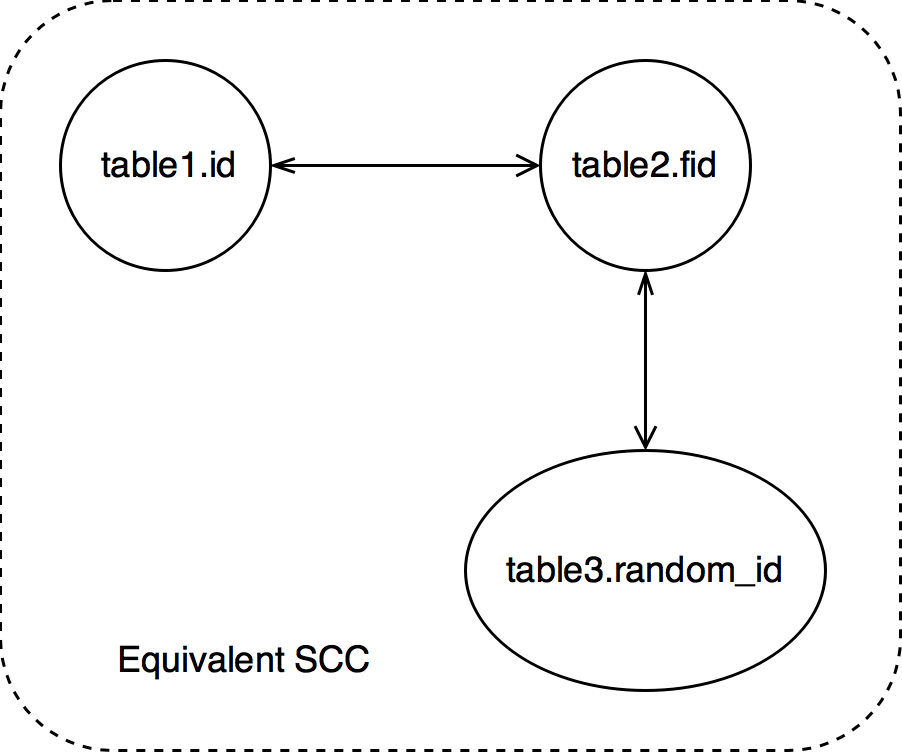
\includegraphics[height=4cm]{Chapters/5-Implementation/scc.png}}
\end{tabular}
\caption{Example of equivalence graph}
\end{figure}

To build the graph we use a Ruby library called RGL. RGL provides the implementation of various graph structures and graph algorithms (including the SCC algorithm).

\begin{listing}
\begin{minted}{ruby}
equivalence = equivalences_list.detect do |equivalences|
  equivalences.include?(column.to_sql)
end

if equivalence.present?
  # transform qualified columns in sql form to two strings representing the
  # table and the column name
  table_name, column_name = equivalence.sort.first.remove("`").split(".")

  SQLParser::Statement::QualifiedColumn.new(
    SQLParser::Statement::Table.new(table_name),
    SQLParser::Statement::Column.new(column_name)
  )
else
  column
end
\end{minted}
\caption{Transforming equivalent columns}
\end{listing}

\subsection{Making defaults explicit}

Every \texttt{MySQL} query has certain default attributes. For instance, every \texttt{MySQL SELECT} query has a default uniqueness filter of \mintinline{mysql}{ALL}. That means while explicitly mentioning \mintinline{mysql}{ALL} will have no effect, it does not mean that it is making the query wrong.

In order to accurately compare two queries, we must make the defaults explicit in both queries.

\subsection{Transforming conditions from WHERE and HAVING}
Both the WHERE and HAVING clauses are represented by a Boolean expression tree. When transforming these clauses it is essential to ensure that the structure of the expression is not altered - that is the before and after expressions are equivalent. To do this, the algorithm traverses the tree recursively and only replaces leafs with either another leaf (in the case of transforming a condition to another) or to a inner node that has two leaves (in the case of transforming a condition to multiple another).

\begin{listing}
\begin{minted}{ruby}
def transform_between_queries(statement)
  if statement.is_a?(SQLParser::Statement::SearchCondition)
    statement.class.new(
      transform_between_queries(statement.left),
      transform_between_queries(statement.right)
    )
  elsif statement.is_a?(SQLParser::Statement::Between)
    transform_between_query(statement)
  else
    statement
  end
end
\end{minted}
\caption{Example of traversing the tree}
\end{listing}

\subsubsection{Transforming conditions with }
\subsubsection{Transforming \mintinline{mysql}{NOT}}
\subsubsection{Transforming \mintinline{mysql}{>}}


\subsection{Implementing transformations}

\section{Partial grading}

\section{Web application user management}
\subsection{Authentication}
Web application is implemented using the devise library. Devise is the most popular authentication library built for Ruby on Rails with over 18000 stars on GitHub and over 33 million downloads on Ruby gems. In addition to a simple login/ logout functionality, devise provides many features out of the box: recovering password, sending and handling confirmation emails, integration with OAuth providers such as Facebook login, etc. An important aspect of any authentication system is how the password are stored in the database. Devise uses the bcrypt algorithm to hash passwords. bcrypt is a password hashing function \citep{wiki:bcrypt} that is used in OpenBSD and Suse Linux and trusted by many big companies such as Dropbox \citep{dropbox:authentication}, in addition to the users of devise and other authentication libraries.

\subsection{Authorization}
To handle roles the application uses two tools: a role field on the user database, and the pundit library. pundit is a library that provides ''authorization through Object Oriented Design and pure Ruby classes'' \citep{github:pundit}. Every user has a role that is either student or admin.

Pundit defines the concept of policies which describe the authorization policy for a model. That means that every model will have an associated policy. A policy has the following attributes:

\begin{itemize}
    \item A policy is instantiated in the controller with the current user and optionally with an instance of an object.
    \item The pundit policy files define methods whose naming convention follows the Ruby on Rails controller action names described in section: \ref{ch:design:web:controller}. That means that a policy defines the following methods: \mintinline{ruby}{def index?}, \mintinline{ruby}{def show?}, \mintinline{ruby}{def create?}, \mintinline{ruby}{def new?}, \mintinline{ruby}{def update?}, \mintinline{ruby}{def edit?}, \mintinline{ruby}{def destroy?}. The method returns whether the user has access to perform the action. An example of this can be seen in listing \ref{fig:policy_challenge}, which makes it clear that only admins can crete new challenges.

\begin{listing}
\begin{minted}{ruby}
class ChallengePolicy < ApplicationPolicy
  # ...
  def create?
    user.admin?
  end
  # ...
end
\end{minted}
\caption{Example policy for Challenge creation}
\label{fig:policy_challenge}
\end{listing}
    \item The pundit method provides the authorize a authorize method to a Ruby on Rails controllers that automatically instantiates a policy, and automatically calls the correct method. An example of the usage of the authorize method is seen in listing \ref{fig:policy_challenge_usage} where the authorize method is called to ensure that the user has access to the challenge. If the user is not authorized, then a response with HTTP code 403 is returned to the user (HTTP code 403 means status is ''Forbidden'').
\begin{listing}[H]
\begin{minted}{ruby}
def show
  @challenge = Challenge.find_by!(id: params.require(:id))
  authorize @challenge
  # ...
end
\end{minted}
\caption{Example of policy usage}
\label{fig:policy_challenge_usage}
\end{listing}
\end{itemize}

\section{Testing}

Testing any software is an essential step in the development process. The purpose of software testing is to validate that the software is behaving as intended \citep{lit:software_testing}. Testing can also be used to check if the requirements have been correctly implemented. As previously mentioned in the development process section (\ref{ch:reqandspec:sec:spec:subsec:dev_process}), testing has been an integral part of the project, with new tests written for all new features added.

Testing is especially important in dynamic languages like Ruby where due to the lack of types and a compile step. Ruby uses what is sometimes called \textit{duck typing} which is enforced using the duck test: ''If it walks like a duck and it quacks like a duck, then it must be a duck.'' \citep{wiki:duck_typing}. That means that Ruby only cares if an object implements a method, it does not care about the type of the object on which the method is called. While this might help developers move faster, duck typing can lead to an increased amount of errors as no type checking is done until runtime. In addition, without a proper test suite, refactoring can become a nightmare for someone working in a dynamic programming language as he has no confidence that the changes he is making will not affect the application.

To ensure that the software is working according to the requirements and that future refactors will be made easily, the project uses two types of testing: unit testing and integration testing.


\subsection{Unit testing}

Unit testing refers to the testing of individual units of code or groups
of related units \citep{unit_testing}. The purpose of unit testing is to
make sure the code meets the specifications \citep{Olan2003}.


In order to unit test the two parts of the application, we are using RSpec which is a DSL testing tool for Ruby \citep{wiki:rspec}.

\subsection{Integration testing}
